\documentclass[a4paper,12pt]{article}

\usepackage[T2A]{fontenc}
\usepackage[utf8]{inputenc}
\usepackage[russian]{babel}

\usepackage[left=25mm,right=15mm,top=20mm,bottom=20mm]{geometry}
\usepackage{graphicx}
\usepackage{amsmath,amssymb,amsthm}
\usepackage{fancyhdr}
\setlength{\headheight}{15pt}

\usepackage{cite}
\usepackage{verbatim}
\usepackage{multirow}
\usepackage[hidelinks]{hyperref}

\pagestyle{fancy}
\fancyhf{}
\fancyhead[R]{Математические формулы}
\fancyfoot[C]{\thepage}

\renewcommand{\theequation}{\arabic{equation}}

\begin{document}
\tableofcontents
\thispagestyle{empty}
\newpage
\section{Математические формулы}

\subsection{Алгебраические и тригонометрические формулы}
\vspace{15pt}
\textbf{Формула \ref{f1}.}
Разложение разности нечётных степеней на множители.

\begin{equation}
\begin{split}
x^{2n+1}-y^{2n+1}&=(x-y)(x^{2n}+x^{2n-1}y+x^{2n-2}y^2+\cdots+y^{2n}) \\
&=(x-y)\left(x^2-2xy\cos\frac{2\pi}{2n+1}+y^2\right)\left(x^2-2xy\cos\frac{4\pi}{2n+1}+y^2\right) \\
&\qquad \cdots\left(x^2-2xy\cos\frac{2n\pi}{2n+1}+y^2\right)
\end{split}
\label{f1}
\end{equation}


\vspace{15pt}
\textbf{Формула \ref{f2}.}
Биномиальный коэффициент и его основные представления.

\begin{equation}
\binom{n}{k}=\frac{n(n-1)(n-2)\cdots(n-k+1)}{k!}=\frac{n!}{k!(n-k)!}=\binom{n}{n-k}
\label{f2}
\end{equation}


\vspace{15pt}
\textbf{Формула \ref{f3}.}
Разложение нечётной степени синуса через синусы кратных углов.

\begin{equation}
\sin^{2n-1} A=\frac{(-1)^{n-1}}{2^{2n-2}}\left\{\sin(2n-1)A-\binom{2n-1}{1}\sin(2n-3)A+\cdots+(-1)^{n-1}\binom{2n-1}{n-1}\sin A\right\}
\label{f3}
\end{equation}


\vspace{15pt}
\textbf{Формула \ref{f4}.}
Сумма арифметико-геометрической прогрессии вида $(a+nb)x^n$.

\begin{equation}
\sum_{n=0}^{N} (a+nb)x^n=\frac{a-(a+bN)x^{N+1}}{1-x}+
\frac{bx(1-x^N)}{(1-x)^2},\qquad (x \ne 1)
\label{f4}
\end{equation}

\vspace{15pt}
\textbf{Формула \ref{f5}.}
Биномиальная формула Ньютона для произвольной степени. \cite{art1}

\begin{equation}
(a+b)^n=\sum_{k=0}^{n}\binom{n}{k}a^{n-k}b^k=a^n+\binom{n}{1}a^{n-1}b+\binom{n}{2}a^{n-2}b^2+\cdots+b^n
\label{f5}
\end{equation}


\subsection{Комплексные числа}
\vspace{15pt}
\textbf{Формула \ref{f6}.}
Деление комплексных чисел путём умножения на сопряжённое число.

\begin{equation}
\frac{a+bi}{c+di}=\frac{a+bi}{c+di}\cdot\frac{c-di}{c-di}=\frac{ac+bd}{c^2+d^2}+\left(\frac{bc-ad}{c^2+d^2}\right)i
\label{f6}
\end{equation}


\vspace{15pt}
\textbf{Формула \ref{f7}.}
Формула Муавра для возведения комплексного числа в степень.

\begin{equation}
(\cos\theta+i\sin\theta)^n=\cos(n\theta)+i\sin(n\theta)
\label{f7}
\end{equation}


\vspace{15pt}
\textbf{Формула \ref{f8}.}
Разложение комплексной экспоненты через степенной ряд.

\begin{equation}
\begin{split}
e^{ix}&=1+ix+\frac{(ix)^2}{2!}+\frac{(ix)^3}{3!}+\frac{(ix)^4}{4!}+\cdots\\
&=\left(1-\frac{x^2}{2!}+\frac{x^4}{4!}-\cdots\right)+i\left(x-\frac{x^3}{3!}+\frac{x^5}{5!}-\cdots\right)\\
&=\cos x+i\sin x
\end{split}
\label{f8}
\end{equation}


\subsection{Интегральные формулы}
\vspace{15pt}
\textbf{Формула \ref{f9}.}
Интеграл функции, содержащей квадратный корень.

\begin{equation}
\int \frac{du}{u\sqrt{a^2-u^2}}=-\frac{1}{a}\ln\left(\frac{a+\sqrt{a^2-u^2}}{u}\right)
\label{f9}
\end{equation}


\vspace{15pt}
\textbf{Формула \ref{f10}.}
Рекуррентные соотношения для интеграла вида $\int x^m(ax+b)^n\,dx$.

\begin{equation}
\int x^m(ax+b)^n\,dx=\begin{cases}\dfrac{x^{m+1}(ax+b)^n}{m+n+1}
+\dfrac{nb}{m+n+1}\int x^m(ax+b)^{n-1}\,dx, \\[10pt]\dfrac{x^m(ax+b)^{n+1}}{(m+n+1)a}
-\dfrac{mb}{(m+n+1)a}\int x^{m-1}(ax+b)^n\,dx, \\[10pt]
-\dfrac{x^{m+1}(ax+b)^{n+1}}{(n+1)b}
+\dfrac{m+n+2}{(n+1)b}\int x^m(ax+b)^{n+1}\,dx.
\end{cases}
\label{f10}
\end{equation}


\vspace{15pt}
\textbf{Формула \ref{f11}.}
Интеграл рациональной функции, представленный через тригонометрические суммы и логарифм.

\begin{equation}
\begin{split}
\int \frac{x^{p-1}\,dx}{x^{2m}+a^{2m}}&=\frac{1}{m a^{2m-p}}\sum_{k=1}^{m}
\sin\left(\frac{(2k-1)p\pi}{2m}\right)\tan^{-1}\left(\frac{x+a\cos\left(\frac{(2k-1)\pi}{2m}\right)}
{a\sin\left(\frac{(2k-1)\pi}{2m}\right)}\right)\\[8pt]
&\quad-\frac{1}{2m a^{2m-p}}\sum_{k=1}^{m}\cos\left(\frac{(2k-1)p\pi}{2m}\right)
\ln\left(x^2+2ax\cos\left(\frac{(2k-1)\pi}{2m}\right)+a^2\right)
\end{split}
\label{f11}
\end{equation}


\subsection{Ряды и специальные формулы}
\vspace{15pt}
\textbf{Формула \ref{f12}.}
Формула Эйлера-Маклорена.

\begin{equation}
\begin{split}
\sum_{k=1}^{n-1} F(k)&=\int_0^n F(k)\,dk-\frac{1}{2}\{F(0)+F(n)\}\\[6pt]&\quad
+\frac{1}{12}\{F'(n)-F'(0)\}-\frac{1}{720}\{F'''(n)-F'''(0)\}\\[6pt]&\quad+\frac{1}{30240}\{F^{(v)}(n)-F^{(v)}(0)\}
-\frac{1}{1209600}\{F^{(vii)}(n)-F^{(vii)}(0)\}\\[6pt]&\quad+\cdots+(-1)^{p-1}\frac{B_p}{(2p)!}
\{F^{(2p-1)}(n)-F^{(2p-1)}(0)\}+\cdots
\end{split}
\label{f12}
\end{equation}


\vspace{15pt}
\textbf{Формула \ref{f13}.}
Полный эллиптический интеграл второго рода и его разложение в ряд.

\begin{equation}
\begin{split}
E=E\left(k,\frac{\pi}{2}\right)&=\int_{0}^{\pi/2}\sqrt{1-k^2\sin^2\theta}\,d\theta=
\int_{0}^{1}\frac{\sqrt{1-k^2v^2}}{\sqrt{1-v^2}}\,dv\\[8pt]&=\frac{\pi}{2}\left\{1
-\left(\frac{1}{2}\right)^2k^2-\frac{1\cdot3}{2\cdot4}\frac{k^4}{3}-\frac{1\cdot3\cdot5}{2\cdot4\cdot6}\frac{k^6}{5}
-\cdots\right\}
\end{split}
\label{f13}
\end{equation}


\vspace{15pt}
\textbf{Формула \ref{f14}.}
Разложение функции в ряд Фурье.

\begin{equation}
f(x)=\frac{a_0}{2}+\sum_{n=1}^{\infty}\left(a_n\cos nx+b_n\sin nx\right)
\label{f14}
\end{equation}


\vspace{15pt}
\textbf{Формула \ref{f15}.}
Бесконечное произведение для гиперболического косинуса.

\begin{equation}
\cosh x=\left(1+\frac{4x^2}{\pi^2}\right)\left(1+\frac{4x^2}{9\pi^2}\right)\left(1+\frac{4x^2}{25\pi^2}\right)\cdots
\label{f15}
\end{equation}


\vspace{15pt}
\textbf{Формула \ref{f16}.}
Бесконечное произведение Валлиса.

\begin{equation}
\frac{\pi}{2}=\frac{2\cdot2}{1\cdot3}\cdot\frac{4\cdot4}{3\cdot5}\cdot\frac{6\cdot6}{5\cdot7}\cdot\frac{8\cdot8}{7\cdot9}\cdots
\label{f16}
\end{equation}


\subsection{Дифференциальные формулы}
\vspace{15pt}
\textbf{Формула \ref{f17}.}
Основные правила дифференцирования.

\begin{equation}
(uv)'=u'v+uv', \quad \left(\frac{u}{v}\right)'=\frac{u'v-uv'}{v^2}
\label{f17}
\end{equation}

%ссылка на таблицу
\vspace{15pt}
\textbf{Формула \ref{f18}.}
Производная сложной функции. Производные элементарных функций приведены в таблице \ref{tab:1}.
\begin{equation}
\frac{d}{dx}f(g(x))=f'(g(x))\cdot g'(x)
\label{f18}
\end{equation}


\vspace{15pt}
\textbf{Формула \ref{f19}.}
Производные степенной, показательной и логарифмической функций.
\begin{equation}
\frac{d}{dx}x^n=nx^{n-1}, \quad \frac{d}{dx}e^x=e^x, \quad \frac{d}{dx}\ln x=\frac{1}{x}
\label{f19}
\end{equation}


\vspace{15pt}
\textbf{Формула \ref{f20}.}
Производные тригонометрических функций.
\begin{equation}
(\sin x)'=\cos x, \quad (\cos x)'=-\sin x, \quad (\tan x)'=\frac{1}{\cos^2 x}
\label{f20}
\end{equation}


\vspace{15pt}
\textbf{Формула \ref{f21}.}
Производные обратных тригонометрических функций.
\begin{equation}
(\arcsin x)'=\frac{1}{\sqrt{1-x^2}}, \quad (\arccos x)'=-\frac{1}{\sqrt{1-x^2}}
\label{f21}
\end{equation}


%таблица
\begin{table}[!h]
\centering
\caption{Таблица производных элементарных функций}
\label{tab:1}
\vspace{15pt}
\begin{tabular}{|c|c|c|}
\hline
\textbf{Вид функции} & \textbf{Функция} & \textbf{Ее производная} \\
\hline

\multirow{3}{*}{Алгебраические} 
& $x^n$ & $nx^{n-1}$ \\ \cline{2-3}
& $\frac{1}{x}$ & $-\frac{1}{x^2}$ \\ \cline{2-3}
& $\sqrt{x}$ & $\frac{1}{2\sqrt{x}}$ \\
\hline
\multirow{3}{*}{Показательные и логарифмические}
& $e^x$ & $e^x$ \\ \cline{2-3}
& $\ln x$ & $\frac{1}{x}$ \\ \cline{2-3}
& $a^x$ & $a^x \ln a$ \\
\hline
\multirow{3}{*}{Тригонометрические}
& $\sin x$ & $\cos x$ \\ \cline{2-3}
& $\cos x$ & $-\sin x$ \\ \cline{2-3}
& $\tan x$ & $\frac{1}{\cos^2 x}$ \\
\hline
\end{tabular}
\end{table}


%setcounter
\vspace{15pt}
\setcounter{equation}{30}

\textbf{Формула \ref{f22}.}
Производная показательной функции с основанием $a$.
\begin{equation}
\frac{d}{dx}a^x=a^x \ln a
\label{f22}
\end{equation}

%картинка + ссылка на книгу
\begin{figure}[!h]
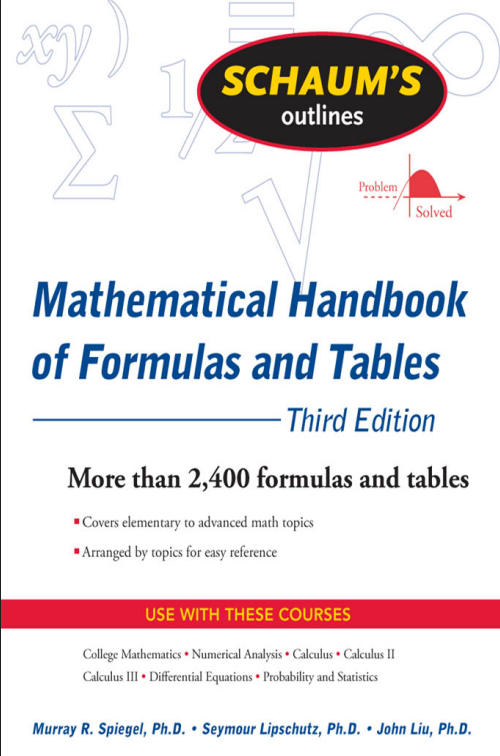
\includegraphics{photo.png}
\centering
\caption{Обложка книги \cite{art1}}
\label{r1}
\end{figure}

%список литературы
\clearpage
\phantomsection
\addcontentsline{toc}{section}{Список литературы}
\begin{thebibliography}{9}
\bibitem{art1} Mathematical Handbook of Formulas and Tables (Third Edition) 
\bibitem{art2} Standard Mathematical tables and formulae (31st edition) - Daniel Zwillinger
\bibitem{art3} Handbook of Mathematical Functions - Abramowitz \& Stegun
\end{thebibliography}
\end{document}
